 \chapter{Arquitetura}
\label{sec:arquitetura}

A arquitectura é uma etapa fundamental em todos os projecto porque é aqui que se define a estrutura e comportamento do sistema na sua globalidade e nas diferentes componentes.

Neste capítulo está exposta a arquitectura do 10.quest que servirá de \textit{guideline} para a implementação do projecto. Serão apresentadas diferentes prespectivas para analisar os diferentes aspectos do sistema. É de notar que as componentes a desenvolver pela restante equipa de desenvolvimento não será analisada e apenas será apresentada de forma superficial para fazer a ligação às componentes a desenvolver no ambito do estágio curricular.
Este capítulo é também uma exposição das decisões arquitecturais efectuadas no primeiro semestre, respeitando as restrições técnicas e de negócios.

Por fim será feita uma analise dos riscos envolvidos no desenvolvimento do projecto, o seu impacto e probabilidade de ocurrência e o respectivo plano de mitigação




\section{Analise da Arquitectura}
\label{analisearq}

Na analise da arquitectura serão apresentadas as restrições do projecto, que têm um impacto directo nas decisões de arquitectura, as diferentes prespectivas de arquitetura e as técnologias utilizadas.

\subsection{Restrições Técnicas}
As restrições técnicas são decisões técnicas arquiteturais que devem ser satisfeitas. O Sistema a desenvolver deve respeitar as seguintes restrições:

\textbf{Identificador: RT01}
\newline
\textbf{Título:} Arquitectura REST
\newline
\textbf{Descrição:} A comunicação entre a plataforma a desenvolver e o TCG deve seguir uma arquitectura REST.

\textbf{Identificador: RT02}
\newline
\textbf{Título:} Base de Dados
\newline
\textbf{Descrição:} Os dados utilizados pela aplicação devem ser guardados numa base de dados, visto tratar-se de um grande volume de dados que tem de permanecer organizado. Relativamente aos dados do TCG foi imposto que os dados não sejam duplicados e que esta informação seja acedida através de pedidos HTTP/REST. PostegreSQL\cite{sql} é a base de dados relacional utilizada pela empresa e portanto será também utilizada no desenvolvimento deste projecto.

\textbf{Identificador: RT03}
\newline
\textbf{Título:} Framework Django\cite{django}
\newline
\textbf{Descrição:} A Framework Django é a técnologia utilizada pela empresa para desenvolver aplicações \textit{web} e \textit{\acrshort{saas}}. O uso desta técnologia foi imposta pelo \textit{Product Owner}.

\textbf{Identificador: RT04}
\newline
\textbf{Título:} Plataforma Web
\newline
\textbf{Descrição:} Todas as funcionalidades do sistema devem estar disponíveis através da plataforma web.

\subsection{Restrições de Negócio}
Nesta secção estão descritas as restrições de negócio, que podem ser entendidas com barreiras que a organização deve lutar para executar a sua estratégia. Estas restrições seguintes foram impostas pelo \textit{Product Owner} e devem ser satisfeitas na arquitectura do sistema:

\textbf{Identificador: RN01}
\newline
\textbf{Título:} Programa de Desenvolvimento
\newline
\textbf{Descrição:} O produto deve estar concluido e validado até dia 15 de Junho.



\subsection{\acrfull{mvc}}

A estrutura de um projeto Django é muitas vezes descrito como um projeto \acrshort{mvc}. Como podemos ver na Figura \ref{fig:arq-mvc}, o modelo \acrshort{mvc} é uma arquitectura de sowftare que separa a aplicação em três componentes lógicos principais. Por outras palavras este modelo separa a apresentação dos dados, da lógica que trata das \textit{interfaces} do utilizador, facilitando a programação das diferentes funcionalidades, \textit{debugging} e os testes das mesmas.

\begin{figure}[ht!]
	\begin{center}
		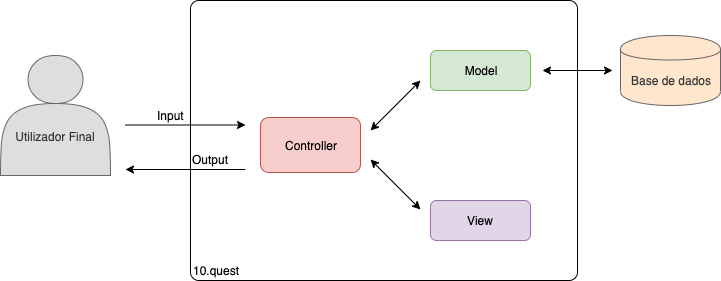
\includegraphics[width=1\textwidth]{img/arq/diagrama-MVC}
		\caption{Estrutura do Sistema}
		\label{fig:arq-mvc}
	\end{center}
\end{figure}

O componente \textbf{\textit{Model}} controla a organização e armazenamento dos dados. Não 


contains only the pure application data, it contains no logic describing how to present the data to a user.

Model represents an object or JAVA POJO carrying data. It can also have logic to update controller if its data changes.

The Model controls the organization and storage of data and may also define
data-specific behavior

The Model component corresponds to all the data-related logic that the user works with. This can represent either the data that is being transferred between the View and Controller components or any other business logic-related data.
\subsection{Modelo C4}


\begin{figure}[ht!]
	\begin{center}
		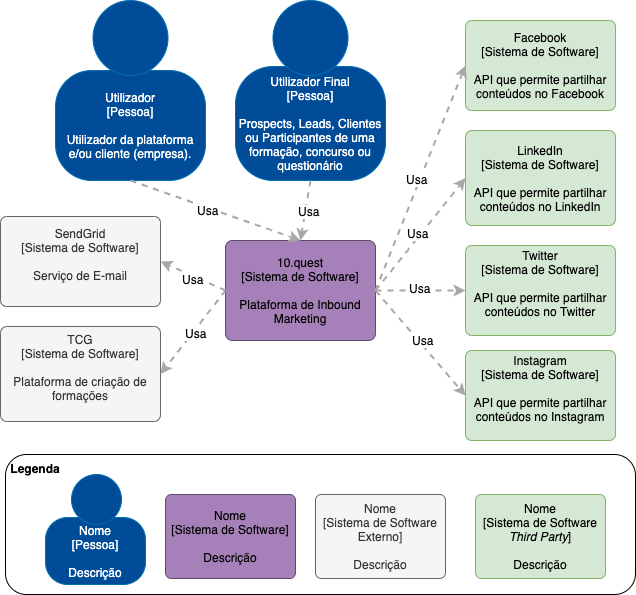
\includegraphics[width=1\textwidth]{img/arq/diagrama-contexto}
		\caption{Diagrama de Contexto}
		\label{fig:arq-contexto}
	\end{center}
\end{figure}

\begin{figure}[ht!]
	\begin{center}
		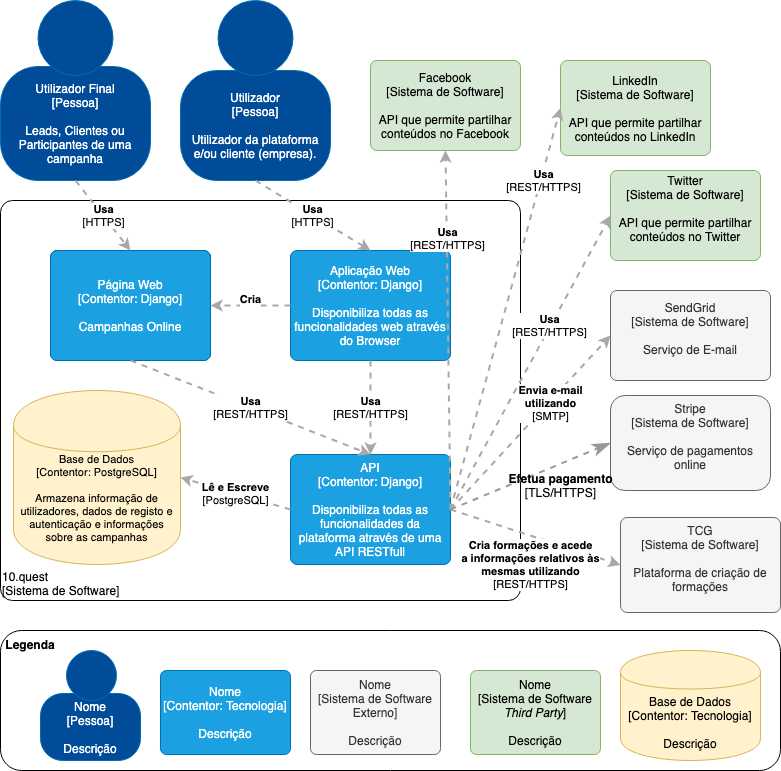
\includegraphics[width=1\textwidth]{img/arq/diagrama-contentores}
		\caption{Diagrama de Contentores}
		\label{fig:arq-contentores}
	\end{center}
\end{figure}

\begin{figure}[ht!]
	\begin{center}
		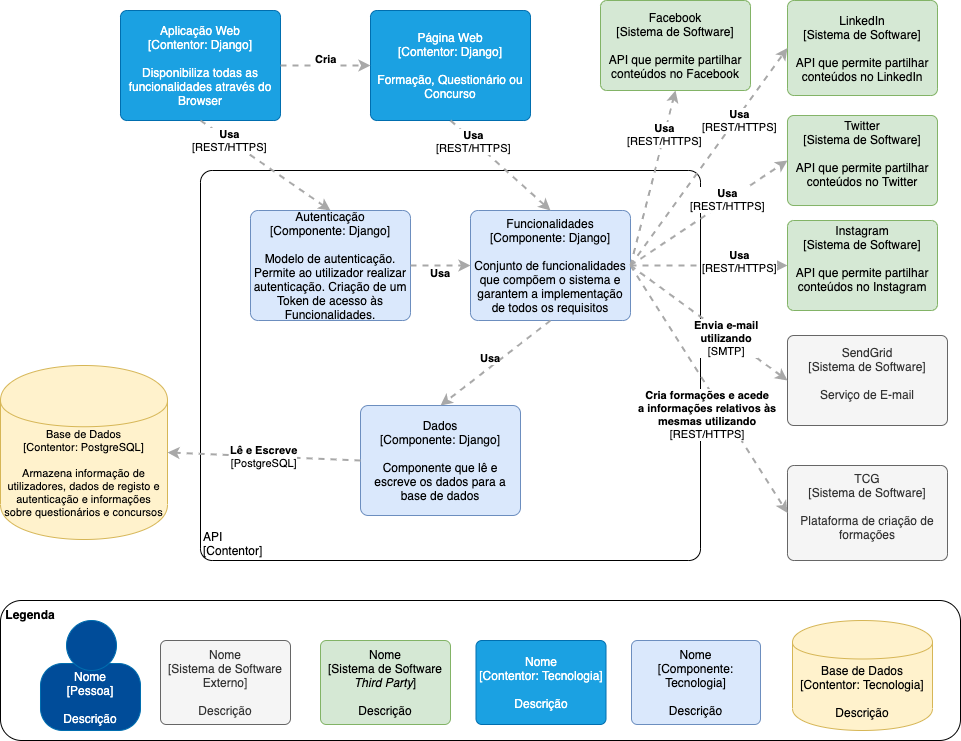
\includegraphics[width=1\textwidth]{img/arq/diagrama-componentes}
		\caption{Diagrama de Componentes}
		\label{fig:arq-componentes}
	\end{center}
\end{figure}

\begin{figure}[ht!]
	\begin{center}
		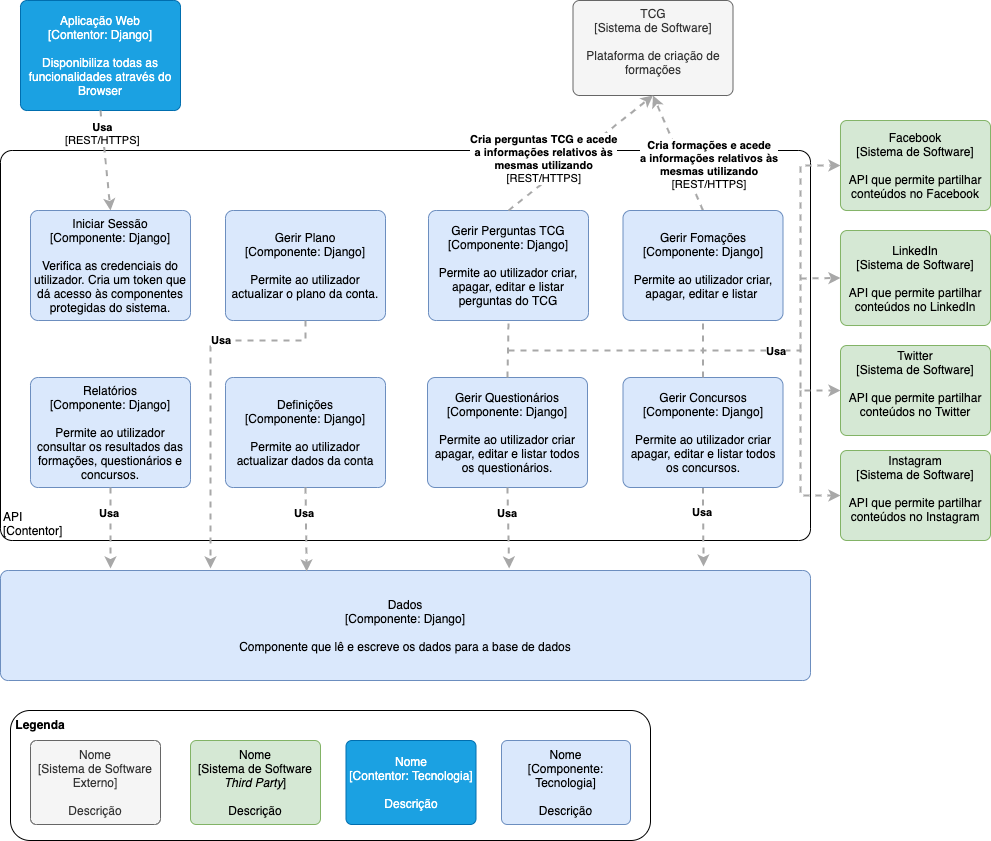
\includegraphics[width=1\textwidth]{img/arq/diagrama-componentes1}
		\caption{Diagrama Componentes da componente Funcionalidades}
		\label{fig:arq-componentes1}
	\end{center}
\end{figure}

\subsection{Modelo Sequencial}

\subsection{Modelo de Dados}

\subsection{Técnologias Utilizadas}

\section{Analise de Riscos}
\label{analiseriscos}
%-------------------------------------------------------------------------------------------------
\blankpage
%-------------------------------------------------------------------------------------------------

\glsresetall
